\section{Effective dynamics}

\begin{frame}{Factorizable dynamics}
    \begin{columns}
        \begin{column}{0.5\textwidth}
            \begin{itemize}
                \item Factorizable unitary dynamics are of the form $\mcU_{t}=\Motimes_{k=1}^{n} U_{k}(t)$.
                Most general effective evolution is
            \begin{equation}
                \boxed{\Gamma_{t}(\rho_{\ef})=\sum_{k=1}^{n}p_{k}e^{-i \omega_{k} H_{k}}\rho_{k}e^{i \omega_{k} H_{k}}.}\nonumber
            \end{equation}
            Non linear!
        \end{itemize}
            \begin{itemize}
                \item Let $H_{k}=\pauli{3}\,\forall\, k$, $\omega_{k}$ be randomly distributed, and $p_{j}\approx\frac{1-p_{1}}{n-1}\,\forall\,j\neq 0$
            \end{itemize}
        \end{column}
        \begin{column}{0.5\textwidth}
            \begin{figure}[h!]
                \centering
                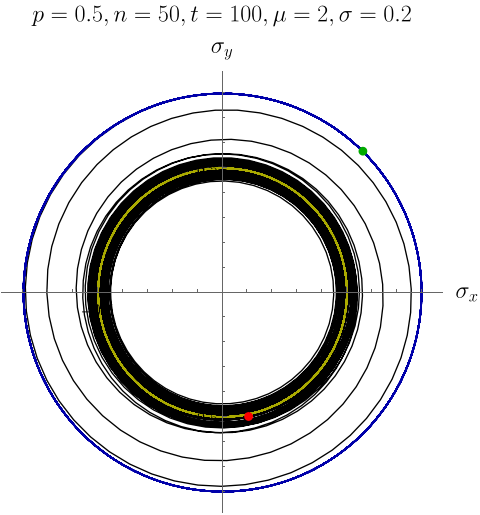
\includegraphics[width=0.7\linewidth]{figures/local_Z_evol_n=50_p=0.5_normal_std=0.2_mean=2_end=100.png}
                \caption{Effective evolution with $\omega_{k}$ normally distributed. }
                \label{fig:SWAPFactor2D}
              \end{figure}
        \end{column}
    \end{columns}
\end{frame}


\begin{frame}{Effective SWAP}
    \begin{columns}
        \begin{column}{0.5\textwidth}
            Effective state before and after:
            \begin{align*}
                \rho_{\ef}(0)&=p_{1}\rho_{1}+p_{2}\rho_{2},\\
                \rho_{\ef}(t=1)&=p_{2}\rho_{1}+p_{1}\rho_{2}.
                \end{align*}
                Contraction!:
                \begin{equation*}
                    \kappa_{t}=\frac{r_{\rho_{\ef}(1)}}{r_{\rho_{\ef}(0)}}.
                  \end{equation*}
                  Non linear depolarizing channel:
                  \begin{equation*}
                      \boxed{\Gamma_{t=1}(\rho_{\ef})=\kappa_{1}^{\rho_{\ef}}\rho_{\ef}+(1-\kappa_{1}^{\rho_{\ef}})\frac{1}{2}\Id.}
                    \end{equation*}
        \end{column}
        \begin{column}{0.5\textwidth}
            \begin{figure}[h!]
                \centering
                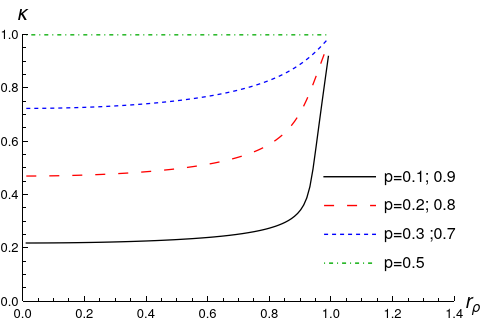
\includegraphics[width=0.9\linewidth]{figures/ContractionFactorSWAP_2D_r0to1_legend.png}
                \caption{Depolarizing coefficient as a function of $r_{\ef}$ for different values of $p$.}
                \label{fig:SWAPFactor2D}
              \end{figure}
        \end{column}
    \end{columns}
\end{frame}

\begin{frame}{Effective Pauli Channels}
    Pauli Channels of $n$ particles are
    \begin{gather}
        P:\mcB(\hilbert_{2^{n}}) \rightarrow \mcB(\hilbert_{2^{n}})\nonumber\\
        P(\Delta)=\sum_{\vec{j},\vec{k}}q_{\vec{j},\vec{k}}\pauli{1}^{\vec{j}}\pauli{3}^{\vec{k}}\Delta\pauli{3}^{\vec{k}}\pauli{1}^{\vec{j}}\rlap{.}\nonumber
    \end{gather}
    where $\pauli{j}^{\vec{k}}=\pauli{j}^{k_{1}}\otimes\pauli{j}^{k_{2}}\otimes ... \otimes \pauli{j}^{k_{n}}$ and $k_{l}\in\{0,1\}$. 
    
    A dephasing channel: $\vec{j}=\vec{0}$ or $\vec{k}=\vec{0}$ and $q_{\vec{j}}=\frac{1-q_{\vec{0}}}{2^{n}-1}\,\forall\,\vec{j}\neq 0$
    \begin{gather}
        P_{\pauli{\nu}}:\mcB(\hilbert_{2^{n}}) \rightarrow \mcB(\hilbert_{2^{n}})\nonumber\\
        P_{\pauli{\nu}}(\Delta)=\sum_{\vec{k}}q_{\vec{k}}\pauli{\nu}^{\vec{k}}\Delta\pauli{\nu}^{\vec{k}}\rlap{,}\nonumber
    \end{gather}
\end{frame}

\begin{frame}{Effective Pauli Channels}
    Applying the coarse graining map to the dephasing channel,
    \begin{align}
        \mcC\qty[\sum_{\vec{j}}q_{\vec{j}}\,\qty(\Motimes_{k=1}^{n} \pauli{\nu}^{j_{k}}\rho_{k}\pauli{\nu}^{j_{k}})]=q_{\vec{0}}\qty(\sum_{k=1}^{n}p_{k}\rho_{k})&+\frac{1-q_{\vec{0}}}{2^{n}-1}(2^{n-1}-1)\qty(\sum_{k=1}^{n}p_{k}\rho_{k})\nonumber\\
        &+\frac{1-q_{\vec{0}}}{2^{n}-1}2^{n-1}\qty(\sum_{k=1}^{n}\pauli{\nu}p_{k}\rho_{k}\pauli{\nu}).\nonumber
    \end{align}
    Effective evolution is a dephasing channel!
    \begin{equation}
        \boxed{\Gamma_{t}(\rho_{\ef})=\qty(q_{\vec{0}}+\frac{2^{n-1}-1}{2^{n}-1}(1-q_{\vec{0}}))\rho_{\ef}+\qty(\frac{2^{n-1}}{2^{n}-1}(1-q_{\vec{0}}))\pauli{\nu}\rho_{\ef}\pauli{\nu}.}\nonumber
    \end{equation}
\end{frame}